\documentclass[11pt,a4paper,english]{uvamath}
\usepackage[english]{babel}

\usepackage{amsmath, amsfonts, amssymb, a4wide, fancyhdr, lineno, graphicx, epsfig, soul, color, hyperref}
\usepackage[square, numbers]{natbib}

% Running line numbers:
\linenumbers
% Number only every 5:th line:
\modulolinenumbers[5]

%Nodig om een bibliography midden in het artikel te zetten, ipv aan het einde zoals eigenlijk gebruikelijk is
\renewcommand{\bibsection}{}

% TODO command
\newcommand{\todo}[1]{
    \hl{#1}
}

% The things that should be filled in by each group, depending on their situation, are written in a todo command, \todo{like this text}. All text in normal the normal font, is applicable for any group. However, everyone is free to adapt any text, and it is even suggested to look at all text critically and make changes if needed.

% Project specific commands
\author{Tom van Duist \& Kevin van den Bekerom}

\newcommand{\projectname}{\todo{Project Name}\ }


\newcommand{\aanpassen}[1]{ {\sethlcolor{green} \hl{#1}} }

\title{Reading assignment week 4}
%Variables
\newcommand{\TitelAbbr}{}
\newcommand{\Version}{0.1}



\what{}
\supervisors{}
\author{Kevin van den Bekerom}


\begin{document}

\maketitle
\clearpage


\chapter*{Reading assignment week 4}

\section*{4.0}
I haven't seen many modeling techniques. I chose some of the more well-defined techniques.

\section*{4.1}

\subsection*{Data Flow Diagram \cite{dfd}}
Graphical represenation of the data flow through an information system. A DFD can also be used in structured design to visualize the data processing steps.
\begin{itemize}
	\item[\textbf{+}] Create overview of system, e.g. find basic functions of Blackboard.
	\item[\textbf{+-}] Great starting point, but not detailed enough.
	\item[\textbf{-}] No formal model, so no validation possible.
\end{itemize}

Example: \\
See Figure \ref{fig:dfd}, A customer can process an order, which is stored in the database, after which credit card data is validated. The order is then shipped. 

\begin{figure}[h]
	\centering
	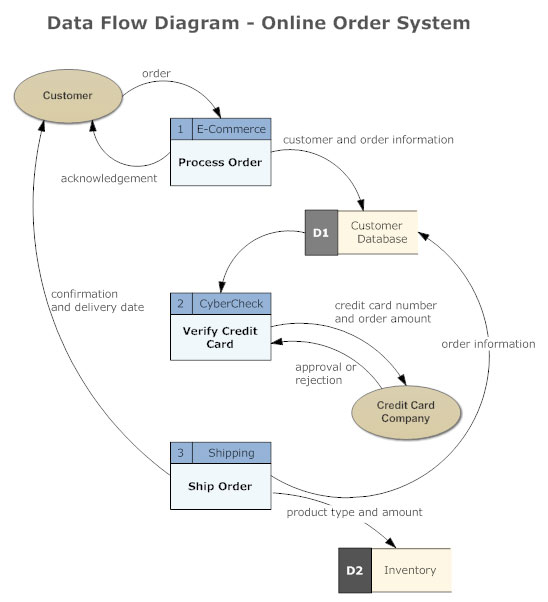
\includegraphics[width=0.75\linewidth]{dfm.jpg}
	\caption{DFD of online order system}
	\label{fig:dfd}
\end{figure}

\subsection*{i* modeling  \cite{i_star}}
Modeling and reasoning about organizational environments and their information systems composed of heterogeneous actors with different, often competing, goals that depend on each other to undertake their tasks and achieve these goals.
\begin{itemize}
	\item[\textbf{+}] Can be used to model both the system-as-is and the system-to-be.
	\item[\textbf{+}] Answers the questions WHY and WHO
	\item[\textbf{+}] Models the goals of the actors (stakeholders). The i* model can be used to derive at a set of important questions to answer during the Requirements Engineering process. 
	\item[\textbf{-}] Does not answer the question HOW?
\end{itemize}

Example:\\
See (Figure \ref{fig:i_star}). In this figure, circles represent actors. Actors have goals (ovals). Goals can have certain quality attributes (soft goals) represented by cloud shapes. Rectangles are resources. A medical researcher has as goal to encrypt data, for which security and privacy are important quality attributes to consider.

\begin{figure}[h]
	\centering
	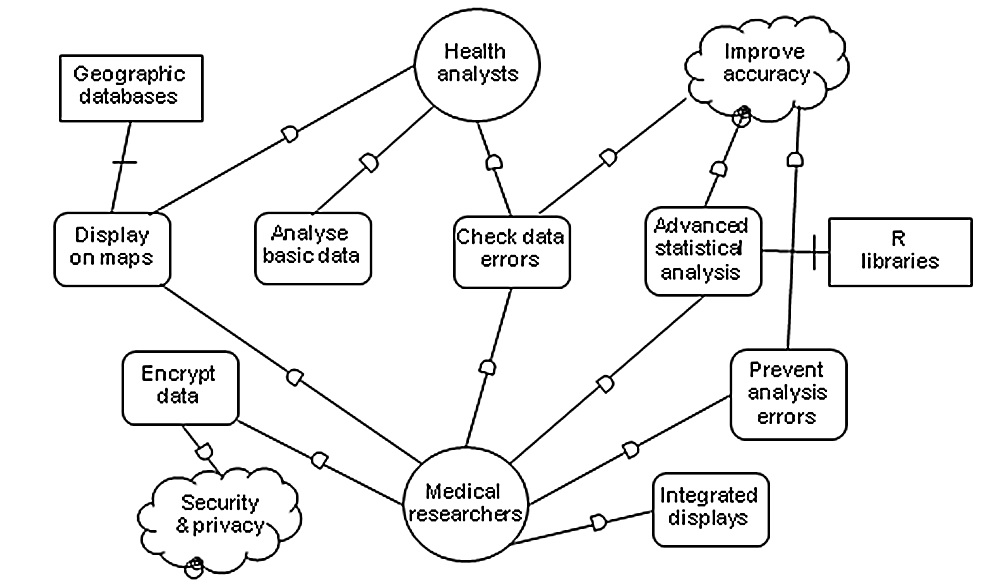
\includegraphics[width=0.75\linewidth]{istar.jpg}
	\caption{i* Diagram for a medical system}
	\label{fig:i_star}
\end{figure}

\clearpage
\subsection*{UI storyboards \cite{ui}}
Model the UI of a system on a high level.
\begin{itemize}
	\item[\textbf{+}] Can be used to ask important usability questions. What are the usability issues Blackboard (can) have. We can categorize these and ask the question if these threaten the goals of certain stakeholders.
	\item[\textbf{-}] High level.
\end{itemize}

Example:\\
See Figure \ref{fig:ui}. In this figure each box is an UI element. Arrows represent data flow between screens. 

\begin{figure}[h]
	\centering
	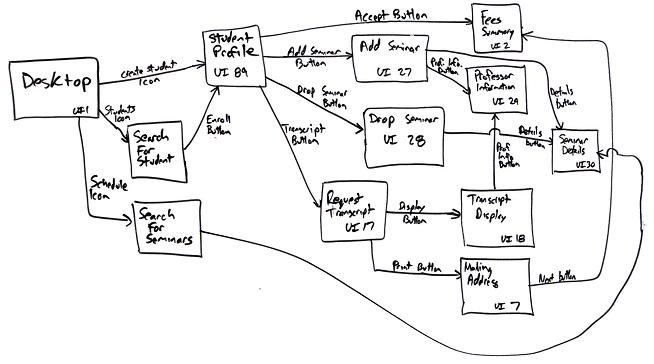
\includegraphics[width=0.75\linewidth]{uiFlow.jpg}
	\caption{UI diagram of university system}
	\label{fig:ui}
\end{figure}

Another good model to organize the information about the Blackboard successor system is the Goal Tree model. In this model we start from a high level goal where multiple stakeholders are involved. Each goal is achieved by achieving subgoals. Gathered information can contribute to achieving a number of goals.

\section*{4.2}
By structuring the data in a Latex document you can make use of hyperlinks. If a new insight makes use of previously gathered data, you can simply make a link to that data. Sections and Chapters can easily be refactored. Using GIT as a content management tool in addition to a latex document creates a logbook, so information is never lost. We have to take care to model data in a modular way, i.e. prevent intertwined, interdependent data. 

\chapter{References}

\begin{thebibliography}{9}
		
	\bibitem{sysml}
	Data Flow Diagram \\
	\url{https://en.wikipedia.org/wiki/Data_flow_diagram}
	
	\bibitem{i_star}
	I* Modeling \\
	\url{https://en.wikipedia.org/wiki/I*}
	
	\bibitem{ui}
	User Interface Flow Diagrams (UI Storyboards): An Agile Introduction \\
	\url{http://www.agilemodeling.com/artifacts/uiFlowDiagram.htm}
	
	
\end{thebibliography}


\appendix


\end{document}
